\documentclass[12pt]{article}

\usepackage[margin=1in]{geometry}
\usepackage{amsfonts, amsmath}
\usepackage{graphicx,wrapfig,subfig}

\newcommand{\R}{\mathbb{R}}
\newcommand{\MOSEY}{\texttt{MOSEY}}

\begin{document}

\begin{titlepage}
	\centering
	\vspace*{\fill}
	{\LARGE\bfseries Random Walks on\\ Simple Two-Dimensional Manifolds\par}
	\vspace{5cm}
	{\large Tom Eichlersmith\par}
	\vspace{5cm}
	An Honors Thesis\par
	Submitted for partial fulfillment of the requirements\par
	for graduation with honors in Mathematics\par
	from Hamline University\par
	\vspace{1em}
	{\today\par}
	\vspace*{\fill}
\end{titlepage}

\section{Introduction}
	The goal of this project was to garner a basic understanding of the mathematics surrounding differential geometry done on two-dimensional surfaces and to produce a computational package that would allow easy exploration of the behavior of walks on these surfaces.
	We will go into more detail of the explanation in the next section; nevertheless, a quick overview of the words in the title is required.
	When we say \emph{random walk}, we intend to construct a series of \emph{steps} on a surface that are each a certain distance a part and the direction of each step is randomly determined. 
	``Simple two-dimensional manifolds" are a set of mathematical objects that mimic the behavior we are used to seeing on the Euclidean plane --- the flat table-top on which we usually study geometry.
	Specifically, they display a ``smooth-ness" that is helpful when attempting to define the distance between two points and the direction of a curve (both of which are needed to define what a step is).
	These random walks are of interest because they are representative of many problems in probability and partial differential equations.
	Moreover, random walks are pretty well understood when they are done on the familiar space of the Euclidean plane; however, questions that are easily answered on the plane cannot be answered when they are extended to other surfaces with different properties.
	
	We will be investigating random walks by studying how long they take to reach a certain region we have defined on the surface.
	We call this destination region the \emph{escape region} and the when a walk enters the escape region we say that it \emph{escapes}.
	In this context, we measure how long a walk takes to escape by calculating the \emph{length} of the walk by simply adding all of the steps from the starting point to the escape region.
	This terminology of ``walking until escaping" is merely a helpful shorthand for our purposes; nevertheless, it implies an application of these mathematics to various modeling problems in biology and population dynamics (some of which explored in \cite{Codling_WalksBiology_2008}).
	Now we will provide a rudimentary understanding of the mathematical tools that are required for our purposes.

\section{Background}
	We must develop machinery in order to replicate the intuitive notion of a walk on different surfaces.
	If we are able to determine what a step is on each of our surfaces, then we define a walk as simply a string of steps connected end-to-end.
	We define a step on a surface as the movement to a point relatively near-by along the shortest path.
	In order to determine this shortest path (as well as the direction the movement is taken), we require computational tools from differential geometry.
	Most of this machinery has been learned from \cite{BanchoffLovett_DiffGeo_2010}.
	The introduction to parametrized surfaces given in \cite{BanchoffLovett_DiffGeo_2010} is most readily adapted to this project because it can be easily implemented in computer programming as opposed to a more abstract approach.
	We will begin with a general overview of differential manifolds that are considered to be ``regular" because of their similarity to what we consider to be intuitively smooth.
	
	\subsection{Regular Surfaces}
		We represent a surface as a subset of $\R^3$ by considering continuous functions $\mu:U \to V$ where $U \subseteq \R^2$ and $V$ is a subset of the surface --- we call the set of $\mu$ that covers the entire surface in question a \textit{chart}.
		Glossing over the large amount of detail and development that can be extracted from this simple idea of a surface, we apply more restrictions on the surfaces (and their charts) in order to obtain an intuitive ``smoothness" on the surface.
		In a sense, these restrictions allow us to consider surfaces that are locally Euclidean (locally plane-like) and therefore they more closely resemble what we perceive a surface to be (hence the name for this class of surfaces).
		Often, a member of the chart for a surface is called a \emph{coordinate patch} because it imposes a relationship between the coordinates of $\R^2$ --- represented by $U$ --- and a part of the surface --- represented by $V$.
		
		For a surface to be \emph{regular}, there must exist a chart that covers the entire surface and has coordinate patches ($\mu$) that each satisfy the following conditions:
		\begin{enumerate}
			\item Differentiable --- the coordinate functions of $\mu$ in $\R^3$ have continuous partial derivatives for all orders
			\item Homeomorphic --- $\mu$ and its inverse are continuous
			\item Satisfies the Regularity Condition --- The differential of $\mu$ is a one-to-one linear transformation
		\end{enumerate}
		When properly constructed, a chart of a regular surface completely characterizes it, and we can calculate all of the properties of the surface we require from the chart.
		Regular surfaces are the only surfaces we will work with in this paper, and are embedded in $\R^3$ by definition.
		Specifically, we choose the Euclidean plane, $P$; the two-dimensional sphere of unit radius, $S$; and the two-dimensional, one-hole torus of polar radius $R$ and axial radius $r$, $T(R,r)$ for study in this project.
		For consistency, we impose the restrictions that all radii are larger than zero and the polar radius of the torus is strictly greater than the axial radius of the torus (i.e. $R > r > 0$).
	
	\subsection{Charts}
		For easier program implementation in C\texttt{++}, we are going to define the charts of our focus surfaces to be slightly different from the usual charts of these surfaces.
		The chart for the Euclidean plane $P$ is the single coordinate patch (the identity patch) $\phi: \R^2 \to P$ defined by
		$$ \phi(u,v) = ( u , v , 0 ) $$
		This is clearly the simplest chart.
		
		The chart for the unit sphere $S$ consists of two (stereographic) coordinate patches, one being $\sigma:\R^2 \to S$ defined by
		$$ \sigma(u,v) = \left( \frac{2u}{1+u^2+v^2} , \frac{2v}{1+u^2+v^2} , \frac{-1+u^2+v^2}{1+u^2+v^2} \right) $$
		The only way to arrive at the north pole $(0,0,1)$ of $S$ using $\sigma$ is to let $u$ and $v$ tend to infinity; thus, another coordinate patch is technically required to define the chart of $S$.
		Practically, the technical need for the other coordinate patch can be ignored when implementing in a computer program because the difficulties arise only at that one infinitesimal point.
		Care can (and will) be taken in order to avoid the issues arising from being on this point.
		For our specific situation, we will always have the north pole contained inside of the escape region so that the walk never needs to arrive at that point. 
		
		Finally, the chart for the torus $T(R,r)$ consists of a single coordinate patch $\tau:I^2 \to T(R,r)$ defined by
		$$ \tau(u,v) = ( (R+r\cos(2\pi v))\cos(2\pi u) , (R+r\cos(2\pi v))\sin(2\pi u) , r\sin(2\pi v) ) $$
		This definition of $\tau$ is easier to implement because its domain is the unit square.
		Computing how to stay in the domain will be easier when the coordinates only have to be compared to $0$ or $1$.\footnote{
			For more detail, investigate the implementation of coordinate wrapping for the torus in \texttt{MOSEY::CoordinateWrappers}. The program would perform less efficiently if it had to compare the coordinates to the approximation of an irrational number on each step.
			Moreover, adding and subtracting an approximated irrational may lead to propagation of error in the program that would not be present otherwise.
			}
		We will use these charts whenever speaking of these surfaces for the rest of this paper, and their form will lead to slightly different calculations that what you see in \cite{BanchoffLovett_DiffGeo_2010,Irons_GeodesicsTorus_2005}.
		
	\subsection{Derivation of Geodesic Equations}
		Geodesics are defined as paths on a surface with no acceleration (relative to the surface).
		This is a method of extending the idea of a line on the plane to other surfaces --- done similarly in \cite{Lewis_GeodesicsMathematica_2002}.
		If $\mu$ represents a coordinate patch on a surface $M$ containing a path $\gamma$, then we can formalize this notion of no acceleration relative to the surface by requiring $\gamma''$ to be normal to the surface everywhere.
		Let $\gamma:[0,1] \to M$, then $\gamma$ is a \emph{geodesic} if
		\begin{equation} \label{geodesic_def} \begin{split}
			&\gamma''(t) \cdot \mu_u = 0 \\
			&\gamma''(t) \cdot \mu_v = 0
		\end{split} \end{equation}
		for all $t$.
		We are able to represent $\gamma(t) = \mu( u(t) , v(t) )$ and expand on this definition to find differential equations for the coordinate functions $u$ and $v$.
		First (omitting the explicit writing of $t$ and writing partial derivatives as subscripts), we have
		\begin{equation*}
			\gamma' = \mu_u u'+\mu_v v'
		\end{equation*}
		and then (using the fact that since $\mu$ is a coordinate patch, we know $\mu_{uv}=\mu_{vu}$ from the first condition)
		\begin{equation*} \begin{split}
			\gamma'' & = (\mu_{uu} u' + \mu_{uv} v')u' + \mu_u u'' + (\mu_{vu} u' + \mu_{vv} v') v' + \mu_v v'' \\
					 & = (u')^2 \mu_{uu} + (v')^2\mu_{vv} + 2u' v'\mu_{uv} + u''\mu_u + v''\mu_v
		\end{split} \end{equation*}
		Now we can put this expression for $\gamma''$ into equation \ref{geodesic_def} to obtain differential equations that the functions $u(t)$ and $v(t)$ must satisfy in order for $\gamma$ to be a geodesic.
		We simplify this substitution by using that $\mu_u$ and $\mu_v$ are orthogonal: $\mu_u \cdot \mu_v = 0$ required by the third condition.
		\begin{equation} \label{geodesic_work} \begin{split}
			\gamma'' \cdot \mu_u & = (u')^2\mu_u \cdot \mu_{uu} + (v')^2\mu_u \cdot \mu_{vv} + 2u' v'\mu_u \cdot \mu_{uv} + u''\mu_u \cdot \mu_u + v''\mu_u \cdot \mu_v \\
			0 & = (u')^2\mu_u \cdot \mu_{uu} + (v')^2\mu_u \cdot \mu_{vv} + 2u' v'\mu_u \cdot \mu_{uv} + u''\mu_u \cdot \mu_u \\
			\gamma'' \cdot \mu_v & = (u')^2\mu_v \cdot \mu_{uu} + (v')^2\mu_v \cdot \mu_{vv} + 2u' v'\mu_v \cdot \mu_{uv} + u''\mu_v \cdot \mu_u + v''\mu_v \cdot \mu_v \\
			0 & = (u')^2\mu_v \cdot \mu_{uu} + (v')^2\mu_v \cdot \mu_{vv} + 2u' v'\mu_v \cdot \mu_{uv} + v''\mu_v \cdot \mu_v \\
		\end{split} \end{equation}
		Rearranging equation \ref{geodesic_work} will be more useful for us. We can assume $\mu_u \cdot \mu_u \neq 0$  and $\mu_v \cdot \mu_v \neq 0$ because of the third condition on $\mu$ we imposed earlier.
		Thus
		\begin{equation} \label{geodesic_eqn} \begin{split}
			u'' + \frac{\mu_{uu} \cdot \mu_u}{\mu_u \cdot \mu_u} (u')^2 + \frac{\mu_{vv} \cdot \mu_u}{\mu_u \cdot \mu_u} (v')^2 + 2\frac{\mu_{uv} \cdot \mu_u}{\mu_u \cdot \mu_u} u'v' & = 0 \\
			v'' + \frac{\mu_{uu} \cdot \mu_v}{\mu_v \cdot \mu_v} (u')^2 + \frac{\mu_{vv} \cdot \mu_v}{\mu_v \cdot \mu_v} (v')^2 + 2\frac{\mu_{uv} \cdot \mu_v}{\mu_v \cdot \mu_v} u'v' & = 0 \\
		\end{split} \end{equation}
		In this form we can pick out the Christoffel Symbols\footnote{
			The Christoffel Symbols are usually defined with respect to the metric tensor on a surface and then the above definition is proven.
			We choose to avoid discussing the metric tensor in order to more directly arrive at the geodesic equations.
			}
		as the coefficients of the derivatives of $u$ and $v$. Specifically,
		\begin{equation}
			\Gamma^i_{jk} = \frac{\mu_{jk} \cdot \mu_i}{\mu_i \cdot \mu_i}
		\end{equation}
		where $i,j,k$ take on the values of $u$ and $v$.
		This ``definition" means we can write equation \ref{geodesic_eqn} in tensor notation
		\begin{equation} \label{geodesic_chris}
			\frac{d^2 x^i}{dt^2} + \sum_{j,k = 1}^2 \Gamma^i_{jk} \frac{d x^j}{dt} \frac{dx^k}{dt} = 0
		\end{equation}
		In \cite{BanchoffLovett_DiffGeo_2010}, equation \ref{geodesic_chris} uses $s$ as the independent variable because these equations produce a geodesic that is parametrized by arc length (has unit speed) when the proper initial conditions are given to it.
		Specifically, if the initial direction vector has unit magnitude, then the resulting solution will have unit speed (and therefore be parametrized by arc length).
		This notation is more compact and highlights the fact that geodesics are determined by the Christoffel symbols and initial conditions.
		
	\subsection{Christoffel Symbols}
		The computer implementation of steps along geodesics uses equation \ref{geodesic_chris}, so we can characterize the geodesics (and therefore walk on the surfaces) by calculating the Christoffel symbols.
		Below are the calculations producing the symbols for each of the coordinate patches from above generated using the CAS \textit{Mathematica}.
		
		The symbols calculated from $\phi$ are quickly obtained.
		Since all of the symbols contain second partial derivatives and $\phi$ only has linear orders of $u$ or $v$, all of the symbols on the plane are zero.
		\begin{equation}
			\begin{array}{lr}
				\left(\Gamma^{u}_{ij}\right) = \left( \begin{array}{cc}
					0 & 0 \\
					0 & 0
				\end{array} \right) &
				\left(\Gamma^{v}_{ij}\right) = \left( \begin{array}{cc}
					0 & 0 \\
					0 & 0
				\end{array} \right)
			\end{array}
		\end{equation}
		
		The coordinate patch $\sigma$ that's a member of the chart of $S$ (and that we will be using for calculations) has the symbols
		\begin{equation}
			\begin{array}{lr}
			\left(\Gamma^{u}_{ij}\right) = \left( \begin{array}{cc}
					-\frac{2u}{1+u^2+v^2} & -\frac{2v}{1+u^2+v^2} \\
					-\frac{2v}{1+u^2+v^2} & \frac{2u}{1+u^2+v^2}
				\end{array} \right) &
			\left(\Gamma^{v}_{ij}\right) = \left( \begin{array}{cc}
					\frac{2v}{1+u^2+v^2} & -\frac{2u}{1+u^2+v^2} \\
					-\frac{2u}{1+u^2+v^2} & -\frac{2v}{1+u^2+v^2}
				\end{array} \right)
			\end{array}
		\end{equation}
		
		The coordinate patch we are using for the torus covers the entire surface with no problematic points (as long as domain wrapping is kept consistent, see below). %REF COORD WRAP SECT
		The Christoffel symbols for $\tau$ are
		\begin{equation}
			\begin{array}{lr}
				\left(\Gamma^{u}_{ij}\right) = \left( \begin{array}{cc}
					0 & -\frac{2\pi r\sin(2\pi v)}{R+r\cos(2\pi v)} \\
					-\frac{2\pi r\sin(2\pi v)}{R+r\cos(2\pi v)} & 0
				\end{array} \right) &
				\left(\Gamma^{v}_{ij}\right) = \left( \begin{array}{cc}
					\frac{2\pi}{r}\sin(2\pi v)(R+r\cos(2\pi v)) & 0 \\
					0 & 0
				\end{array} \right)
			\end{array}
		\end{equation}
		
		These Christoffel symbols for each of the surfaces are finite at every point in their domains.
		This good behavior is helpful when implementing them in the computer program, and it is a result of the choices of coordinate patches we use to study the surfaces.
	
\section{Random Walks}
	Now that we have all of the tools necessary to take steps on each of our three surfaces, we are able to walk on them.
	The implementation of these walks is in C\texttt{++} using an application of the standard Runge-Kutta method to numerically solve the geodesic equations in steps.
	Once we are able to take a single step in any direction and from any point on the surface, we are able to randomly walk on the surface.
	
	For the implementation in C\texttt{++}, we have chosen to have the direction be uniformly random; this choice could be edited by the user in the \texttt{MOSEY::RandDouble} class.
	We walk in different situations; when we reference a \emph{situation}, we are talking about the surface-escape region pair that (we believe) defines the behavior of the walks.
	A general structure to walk on a given surface is constructed in the package \MOSEY{} where one can define a surface by its Christoffel symbols (\texttt{MOSEY::CurveTensor}) and how its coordinates connect across domain edges (\texttt{MOSEY::CoordinateWrappers}).
	This package is designed to study various situations involving regular surfaces and simply defined escape regions.
	The walks are done in the coordinate space and then output to a \texttt{csv}-file in a format depending on the situation --- for example, the walk distances are output with respect to polar angles when walking on the sphere (Section \ref{sphere}).
	
	For each situation, we can explore several questions using the package \MOSEY{}.
	How are the walk lengths and escape regions related?
	How much of an impact does the surface the walk is on have?
	Does the size of the escape region (relative to the surface) have a large effect? The results given below merely scratch the surface of the knowledge that could be garnered from \MOSEY{}.
	
	\subsection{Stepping Method}
		On many surfaces, the geodesic equations \ref{geodesic_chris} are able to be solved analytically --- both $P$ and $S$ have this behavior; however, these analytical solutions do not necessarily allow for an increase in speed.
		Moreover, we would like \MOSEY{} to be constructed generally enough to deal with surfaces that contain geodesics that are more difficult to define analytically like $T(R,r)$.
		Therefore, we have written a method for stepping on surfaces that is a numerical approximation but is also quick and can be used with any set of self-consistent Christoffel symbols.
		
		The Runge-Kutta method is a process to approximate first order differential equations.
		We will be using the standard, fourth order Runge-Kutta method (RK4) that will be outlined for our specific problem below.
		First, we must transform our two second order geodesic equations \ref{geodesic_chris} into a system of first order differential equations so that we are able to apply the RK4 method.
		
		We begin by expanding \ref{geodesic_chris} and using $u$ and $v$ instead of $x^1$ and $x^2$.
		\begin{equation} \label{geodesic_expansion} \begin{split} 
			\frac{d^2u}{dt^2} & = -\Gamma^u_{uu}\left(\frac{du}{dt}\right)^2-2\Gamma^u_{uv}\frac{du}{dt}\frac{dv}{dt}-\Gamma^u_{vv}\left(\frac{dv}{dt}\right)^2 \\
			\frac{d^2v}{dt^2} & = -\Gamma^v_{uu}\left(\frac{du}{dt}\right)^2-2\Gamma^v_{uv}\frac{du}{dt}\frac{dv}{dt}-\Gamma^v_{vv}\left(\frac{dv}{dt}\right)^2 \\
		\end{split} \end{equation}
		Define the first derivatives of $u$ and $v$ as their own variables
		\begin{equation*} \begin{array}{cc}
			p = \frac{du}{dt} & q = \frac{dv}{dt}
		\end{array} \end{equation*}
		Then \ref{geodesic_expansion} becomes the system
		\begin{equation} \begin{split}
			\frac{du}{dt} & = p \\
			\frac{dv}{dt} & = q \\
			\frac{dp}{dt} & = -\Gamma^u_{uu}p^2-2\Gamma^u_{uv}pq-\Gamma^u_{vv}q^2 \\
			\frac{dq}{dt} & = -\Gamma^v_{uu}p^2-2\Gamma^v_{uv}pq-\Gamma^v_{vv}q^2 \\
		\end{split} \end{equation}
		This is a system of first order differential equations, so we can adapt RK4 to numerically solve it.
		
		Define $y = \langle u , v , p , q \rangle$.
		Suppose $(u_0,v_0)$ is the point we wish to step from and we are moving at an angle $\theta$ relative to the positive $u$ axis (at that point).
		Then the initial vector is $y_0 = \langle u_0 , v_0 , \cos(\theta) , \sin(\theta) \rangle$.
		This begins the geodesic with unit speed, meaning that it is parametrized by arc length, so if we wish to step a distance $h$, we numerically solve the initial value problem given by
		\begin{equation} \label{RK4_imp} \begin{split}
			\frac{dy}{dt} & = F(y) = \langle p , q , -\Gamma^u_{uu}p^2-2\Gamma^u_{uv}pq-\Gamma^u_{vv}q^2 , -\Gamma^v_{uu}p^2-2\Gamma^v_{uv}pq-\Gamma^v_{vv}q^2 \rangle \\
			y(0) & = y_0
		\end{split} \end{equation}
		until $t = h$.
		Let $N$ be the number of iterations of the RK4 method we will use to approximate \ref{RK4_imp}.
		Define $\delta = h/N$, then we write our approximation scheme below.
		\begin{equation} \label{RK4_alg} \begin{split}
			& y \gets y_0 \\
			& \textit{loop } N \textit{ times:} \\
			& \quad k_1 \gets F(y) \\
			& \quad k_2 \gets F\left(y+(\delta/2)k_1\right) \\
			& \quad k_3 \gets F\left(y+(\delta/2)k_2\right) \\
			& \quad k_4 \gets F\left(y + \delta k_3\right) \\
			& \quad y \gets y+(\delta/6)(k_1+2k_2+2k_3+k_4)
		\end{split} \end{equation}
		When implemented correctly, the loop exits with $y$ containing an approximate value for $u$, $v$, $p$, and $q$ a distance $h$ away from $(u_0, v_0)$ on the surface.
		This method is constructed in the \texttt{MOSEY::Stepper} class.
	
	\subsection{Coordinate Wrappers}
		The implementation of the walks in \MOSEY{} assumes that there is a single coordinate patch whose range covers the area of the surface that the walks will be contained within.
		Some of the coordinate patches used do not cover the whole surface (e.g. $\sigma$), but as long as the un-covered points are in the escape region, this lack of coverage is not a problem.
		Other coordinate patches have bounded domains (e.g. $\tau$), and in order for there to be a one-to-one relationship between the coordinates in the domain and the points on the surface, we must be careful when a walk attempts to cross the border of the domain.
		The functional class \texttt{MOSEY::CoordinateWrappers} is an attempt to deal with this difficulty.
		Each surface has a ``coordinate wrapper" defined for it that is intended to keep the points within the desired region without affecting the walk.
		Both $\phi$ and $\sigma$ have unbounded domains, so their coordinate wrappers do not edit the walk points; however, $\tau$ is confined to the unit square.
		Studying how $\tau$ is related to the torus, we see that parallel edges are ``glued" together, so if we exit on one side, we need to re-enter on the other side.
		This wrapping is done with simple arithmetic.
		
		Another, unintentional, utility is available through the coordinate wrapper style.
		Some situations require a walk to be reflected off a boundary like the Circular Walls situation on the plane (Section \ref{circwalls}).
		These reflection boundaries, \emph{walls}, can be implemented in this function style for a specific situation by doing calculations on the current and previous step points in the domain.
		
	\subsection{Optimizations}
		In order for the walks on the different surfaces to be efficiently studied, some situations admit specific optimizations, saving computing time.
		We are not claiming these processes to be perfectly optimized (read \cite{Redfield_NumericalGeodesics_2007} for a more detailed exploration of efficient numerical solutions to the geodesic equations), but we wish to explain the methods we have used to make the simulation of walks more efficient.
		
		The first (and most widely applicable) optimization is recording every step of a random walk as if it was the first step of the walk following it.
		This allows for several walks starting from different initial positions to be acquired through one iteration.
		We are able to use this data because steps are independent of their predecessors.\footnote{There are more general random walk problems that deal with steps that are dependent on each other, but this complication would only slow the program down for our purposes. Various modifications could be made in the \MOSEY{} package in order to account for steps that are dependent on previous ones.}
		
		Walks on the plane offer the massive simplification of having all zero Christoffel symbols.
		In order to take a step of length $h$ at an angle $\theta$ from the positive $u$-axis, we could simply add $(h\cos(\theta), h\sin(\theta))$ to the initial point.
		We do not do this directly because we would like uniformity across the code package.
		However, using RK4 with the number of iterations $N = 1$ produces the exact same result algebraically.
		Due to the limited precision of numbers in computers, this equality is not perfect; nevertheless, it produces a result that only differs from the exact result due to inherent truncation errors in the computer (which implementing the exact result would suffer from as well).
		Therefore, when the class \texttt{MOSEY::Stepper} is configured to take a step on $P$, the number of iterations used in RK4 is set to one (overriding any user specifications).
		This avoids unnecessary calculations from additional loops that would not produce a more accurate result.
		
		The two-dimensional sphere is also incredibly symmetrical.
		In this specific situation, the escape regions are generally circles with centers at the north pole.
		Because of the symmetry around the axis of the sphere, we are able to only consider polar angle (the angle the point makes with the north pole) when analyzing how the walk distance changes depending on the starting location.
		We calculate the polar angle $\phi$ of the point $\sigma(u,v)$ by
		\begin{equation*}
			\phi = \arctan\left(\frac{1}{u^2+v^2}\right)
		\end{equation*}
		This simplification will not help the walks themselves be simulated more efficiently; nevertheless, it will allow for the analysis of the data gathered from the walks be simplified --- making it one-dimensional instead of two.
		
		Due to the inherently large amount of noise generated by collecting data in a purely pseudo-random fashion, the general trends that we expect to appear only arise after several hundred (if not more) walks.
		Since each walk is hundreds or even thousands of steps (and each step is treated as its own data point), we are required to have millions of data points collected for each manifold-escape region pair.
		This amount of data leads to an inability to process it all, so we have chosen to compress the data into summary files that are at most one hundred thousand data points.
		The raw data is still stored; nevertheless, these summary files are valuable to construction of plots that would crash under the weight of millions of points.
		The compression method is binning the data into thin bins and determining the mean for each bin.
		This procedure substitutes one data point for a few thousand, which quickens analysis and plotting while maintaining accurate reflection of the data.
		Since this ``compressed means" procedure loses information in the data (specifically, how skewed the data is), we avoid using the compressed means unless absolutely required.
		The instance where we use the compressed means in this report is when plotting several different situations on the sphere in Figure \ref{fig:compsphere} below.

\section{Results}
	The construction of this package has arrived at several results that display the versatility of it.
	While only a small number of concrete situations have been investigated, these investigations have shown that \MOSEY{} is versatile enough to tackle almost any situation defined on the torus, sphere, or plane.
	We will now go into more detail about specific results of this project.\footnote{
		When medians of data are plotted in one-dimension, the first quartile and third quartile are included to give an idea of the breadth of the distribution.
		}
	
	\subsection{Plane}
		First, we began the investigations with a situation that can be solved analytically.
		As stated earlier, the Plane, being the special situation with all zero Christoffel symbols, allows for an easy testing ground for our random walk machinery.
		\begin{figure*}[htp]
			\centering
			\begin{tabular}{p{0.5\textwidth}p{0.5\textwidth}}
				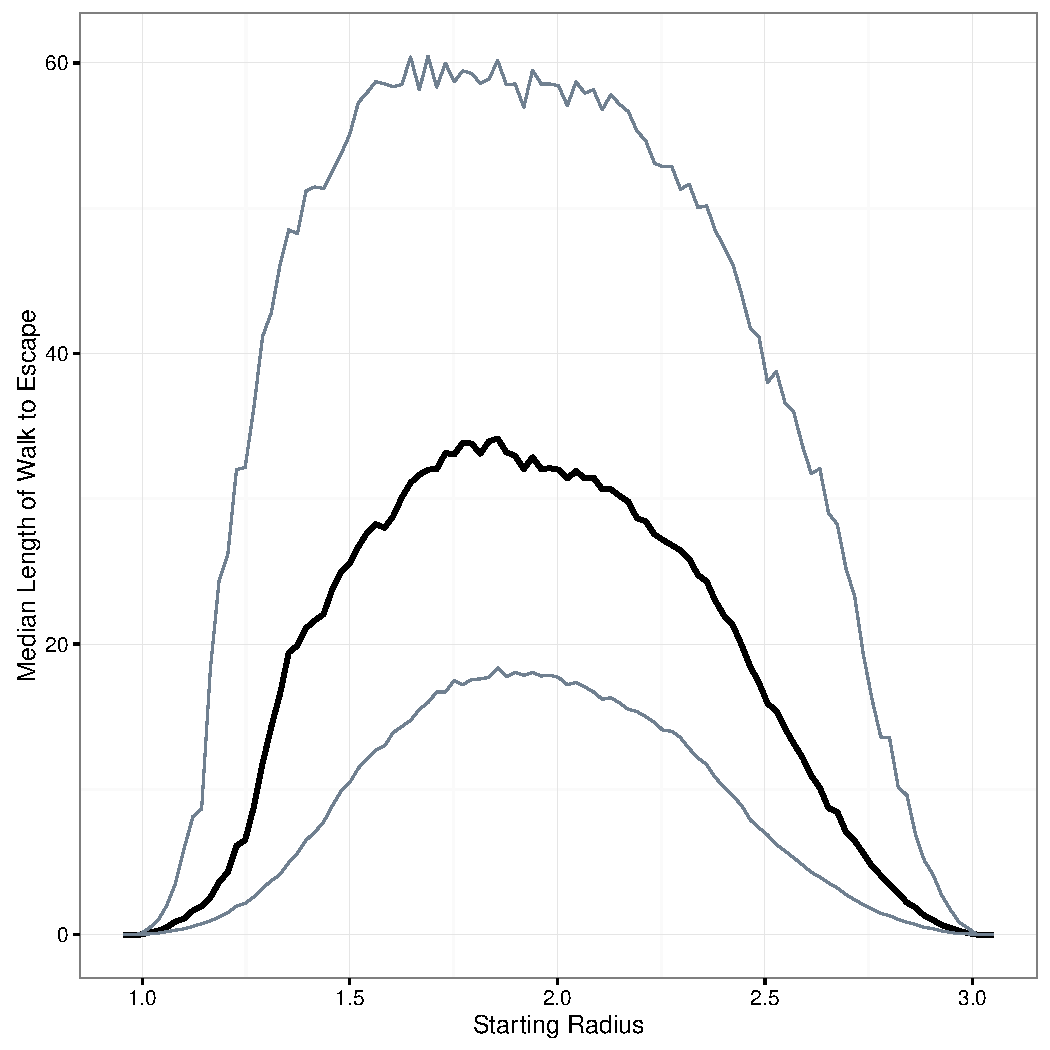
\includegraphics[width=0.48\textwidth]{images/PlaneIn1Out3.pdf}
				\caption{Example data plot from the plane with the escape region beginning at radius $1$ and radius $3$.}
				\label{fig:planering}
				&
				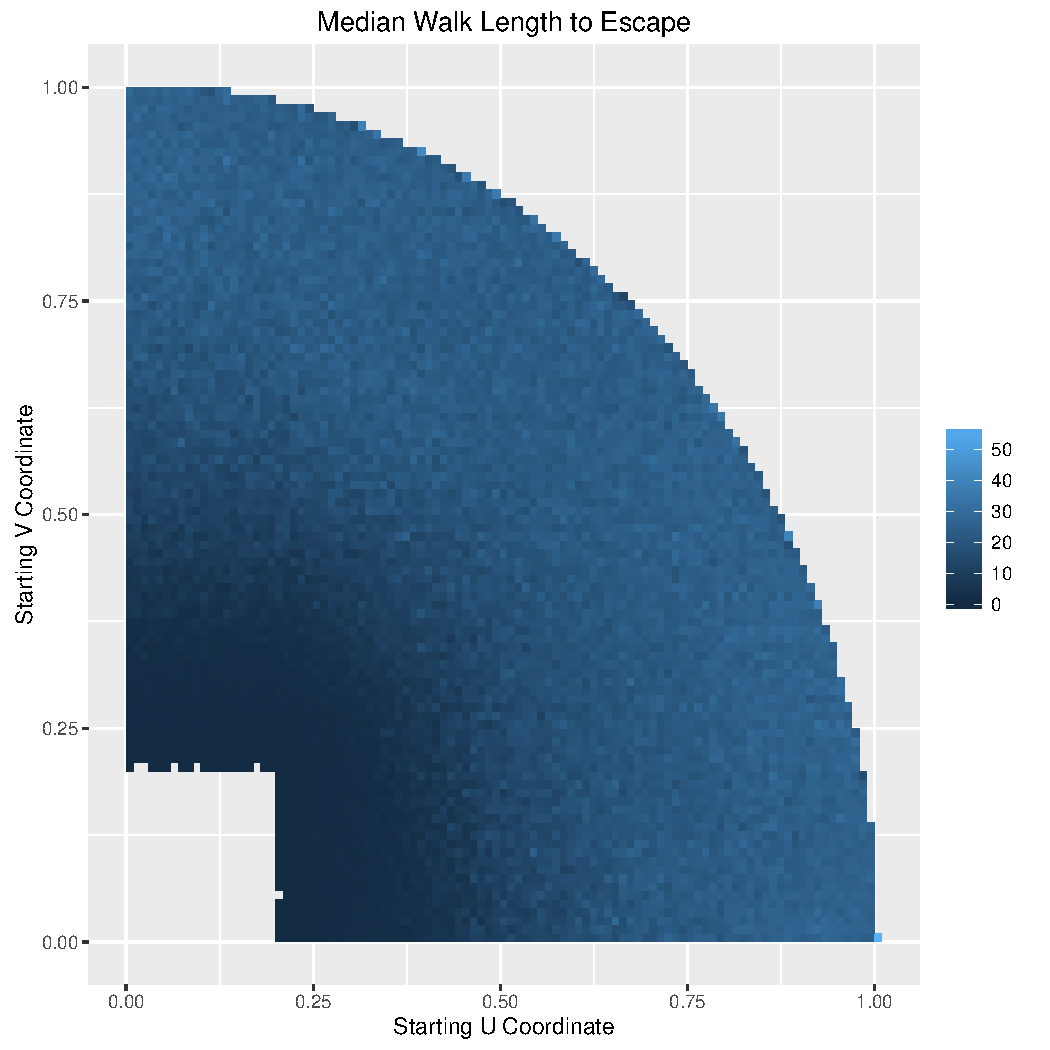
\includegraphics[width=0.48\textwidth]{images/PlaneCircleL05.pdf}
				\caption{Circular Walls example (only the first quadrant is plotted).}
				\label{fig:planecircwalls}
			\end{tabular}
		\end{figure*}
		
		\subsubsection{Ring}
			The ``Ring" situation uses $P$ as the surface and two concentric circles as the border of the escape region.
			If a point is inside the smaller circle or outside the larger cirle, then the walk has escaped.
			This allows for the plane to be bounded in a continuous fashion, and the walks have a radial symmetry, so only the radius-walk length dependence needs to be studied.
			
			The averages over the walks show the expected quadratic dependence that is calculated in the analytical solution.
			This specific situation is wildly inefficient (because there is an analytical solution available); nevertheless, it displays the power of the random walk method.
			This relatively simple computational method allows for determination of numerical solutions to intricate differential equations, and this method has a process that is easy for the user to understand --- more on this discussion in section \ref{NumericSoln}.
			
		\subsubsection{Circular Walls}
			We now extend the method to a situation that is slightly more complex.
			This situation has ``walls" --- borders that the walk bounces off of instead of passing through.
			Moreover, it has an escape region with a non-smooth border.
			The walls are defined as the unit circle around the origin, and the escape region is a square within the walls.
			These two complexities, which offer large resistance in finding the analytical solution, are easily incorporated into this framework.
			Nevertheless, the symmetries in this situation are not enough to simplify the analysis to one dimension, therefore requiring more data to be generated.
			
			Figure \ref{fig:planecircwalls} shows an example for this situation, the square has $0.5$-length sides and is centered on the origin.
			Each bin has the median of the walks starting from inside that bin as its value.
			The behavior in this case is predictable --- the walks approach zero length exponentially as they near the escape region.
			
	\subsection{Sphere} \label{sphere}
		\begin{figure*}[htp]
			\centering
			\begin{tabular}{p{0.5\textwidth}p{0.5\textwidth}}
				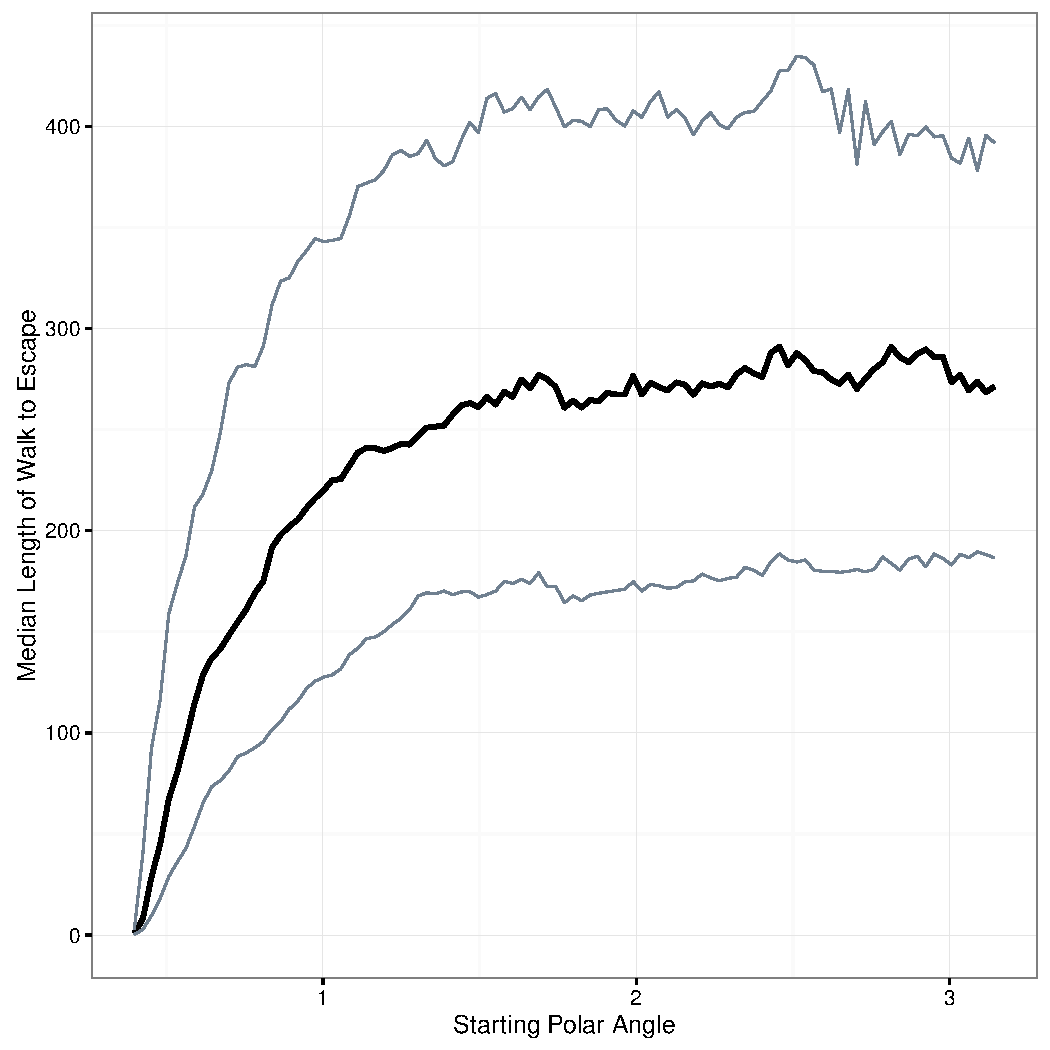
\includegraphics[width=0.48\textwidth]{images/ExampleSphereL04.pdf}
				\caption{Example data plot from the sphere with the escape region beginning at polar angle $0.4$.}
				\label{fig:egsphere}
				&
				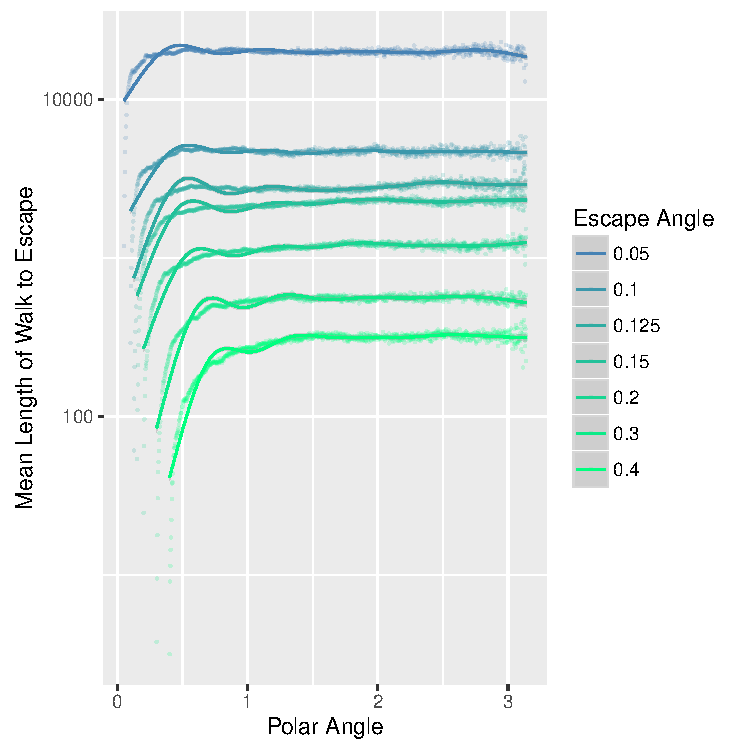
\includegraphics[width=0.48\textwidth]{images/SummaryPlot_L005_04.pdf}
				\caption{Comparison of several situations with different escape angles.}
				\label{fig:compsphere}
			\end{tabular}
		\end{figure*}
		The sphere surface has been studied the most extensively in this project because it is a good compromise between unexplored territory and few output variables.
		Since the escape regions that are studied in these situations are symmetric around the polar axis, we are able to represent the data on the sphere as its angle with respect to the positive z-axis in normal polar coordinates.
		This angular representation allows for the analysis to be done in one-dimension, enabling more precise analysis to be done without requiring that much more data.
		Moreover, the escape regions are also able to be characterized by their border at a certain angle, the \emph{escape angle}.
		
		In Figure \ref{fig:egsphere}, you can see how the length of the escape walk changes depending on the polar angle of the starting point --- this behavior is interesting and appears to be a fractional power dependence.
		Several different sizes of escape regions on the sphere were studied, and the summary of the results can be seen in Figure \ref{fig:compsphere} (using the compressed means instead of the raw data).
		Most importantly, the length of the escape walk from anywhere on the sphere seems to increase exponentially as the escape angle decreases.
	
	\subsection{Torus}
		\begin{figure*}[htp]
			\centering
			\begin{tabular}{p{0.5\textwidth}p{0.5\textwidth}}
				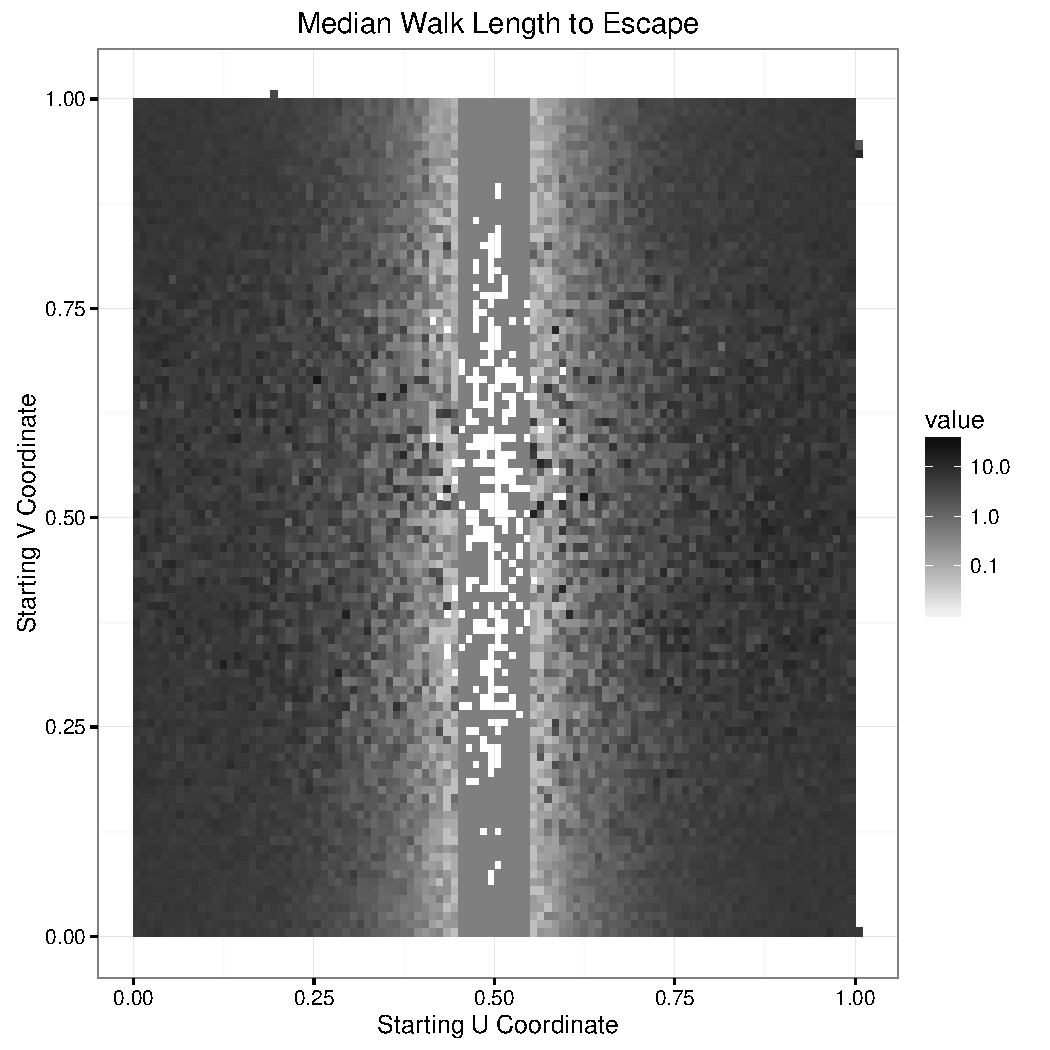
\includegraphics[width=0.48\textwidth]{images/TorusUBand.pdf}
				\caption{Example Torus with the U-band escape region having a width of $0.1$.}
				\label{fig:egtorusU}
				&
				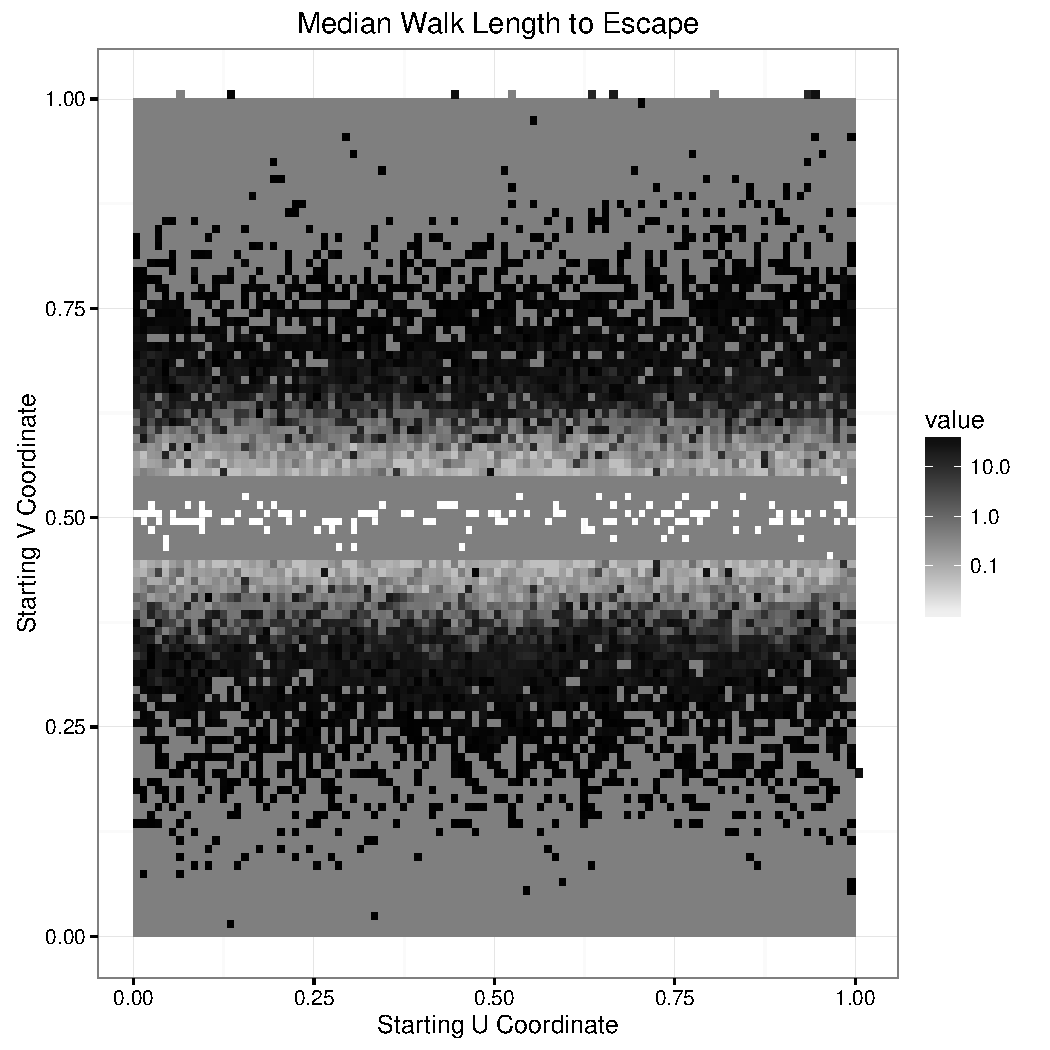
\includegraphics[width=0.48\textwidth]{images/TorusVBand.pdf}
				\caption{Example Torus with the V-band escape region having a width of $0.1$.}
				\label{fig:egtorusV}
			\end{tabular}
		\end{figure*}
		The torus is the surface in this project with the richest structure, and in our specific instance we study $T(2,1)$.
		The walks are assumed to have almost no symmetry involved, so the entire domain of $\tau$ is studied.
		We focus on two different types of escape regions on the torus U-bands and V-bands.
		U-bands are escape regions that contain v coordinates anywhere between $0$ and $1$.
		Similarly, V-bands contain u coordinates anywhere between $0$ and $1$.
		These are rudimentary escape regions to study, but since the behavior of walks on this surface is not very well known, we must begin with the basics.
		
		Figure \ref{fig:egtorusU} displays an example of the situation with a U-band of width $0.1$.
		The placement of this band on torus is not of great importance because of the symmetry in the $u$ coordinate; therefore, we placed the band in the center of the defined domain so the graphic is easier to study.
		Here we can see how the walk shortens exponentially as one approaches the band --- the uniform color aligned with the band in this image is due to the breakdown of the logarithmic scale from lack of data in that region.
		
		Figure \ref{fig:egtorusV} displays a V-band example (of width $0.1$), which is much more interesting.
		The placement of this band on the torus \emph{is} of importance because the curvature of the torus changes in the $v$ coordinate.
		This band was chosen to wrap around the outside of the torus, and one can see that the walks decrease in length when they begin inside of the torus.
		This behavior was unexpected and offers an arena for further exploration.
		
	\subsection{Overall Package}
		Without any more pretty pictures to present, we would like to point out the central product of this project.
		The package \MOSEY{} that was used to simulate these walks on various surfaces is perhaps the most valuable outcome of this project.
		Its structure allows for incorporation of an amazing amount of different situations, meaning that it can be used to quickly generate data for a more detailed study of this escape length problem.
		Moreover, although not required, experience with C\texttt{++} would allow the user to modify any part of the package.
		Even with minimal programming experience, the code and its documentation allows for the user to experiment with different situations, including changing the starting position or the size of the escape region.
		
		This package's most important trait is its flexibility.
		The examples already written into the package attempt to give an idea of what can be done with it.
		Specifically, the \texttt{MOSEY::CoordinateWrapper} function style can be used to define walls (like in the Circular Walls situation) as well as wrap coordinates to maintain domain consistency (like on the torus).
		
	\subsection{Numeric Solution} \label{NumericSoln}
		We end with an example of applying this idea of random walks on different surfaces.
		The convergence of the solution in the Ring situation suggests a relation between averaging random walks in a situation and solving the differential equation $\Delta u = -1$ for the same situation.
		Indeed, the solution to the system
		\begin{equation*} \begin{split} 
			\Delta u(x,y) & = -1 \\
			u(x,y) & = 0 \quad\text{if } x^2+y^2 = 1 \text{ or } x^2+y^2 = 9
		\end{split} \end{equation*}
		gives the quadratic dependence shown in the average of the walks for the given Ring situation.
		This hint of a relationship is exciting because extending $\Delta u = -1$ to other surfaces and escape regions makes determining the solution more difficult, while extending the idea of a random walk is in some sense easier (at least we know how to do it).

\section{Conclusion}
	Personally, this project was able to give me an introductory understanding to simple differential geometry; an understanding that is complex enough to construct numerical approximations of geodesics on various surfaces.
	Moreover, we were able to successfully create a flexible and powerful simulation package in C\texttt{++}: \MOSEY{}.
	\MOSEY{} is able to simulate random walks on various surfaces; the plane, sphere, and torus are already built into its structure.
	Random walks have been studied on these simpler surfaces and interesting behavior has been found.
	The documentation of this package is attached to the github repository that it is stored online, available to the public.\footnote{
		\texttt{github.com/tomeichlersmith/RandomManifoldWalks}
		}
	

\pagebreak
\bibliographystyle{plain}
\bibliography{../../References/References_MathDHP_201718}

\end{document}